\documentclass{article}
\usepackage[margin = 1in]{geometry}
\usepackage{graphicx}
\usepackage{amsmath}
\usepackage{amssymb}
\usepackage{bm}
\usepackage{tcolorbox}
\usepackage{latex-rmd}
\newcommand{\E}{\mathrm{E}}
\newcommand{\Log}{\log}
\renewcommand{\log}{\:\mathrm{log}\:}
\renewcommand\thesubsection{\thesection.\alph{subsection}}
\setlength{\parindent}{0em}
\setlength{\parskip}{1em}

\title{Advanced Macroeconometrics - Assignment 2}
\author{Miriam Frauenlob, Elisabeth Fidrmuc, Tim Koenders }
\date{May 2023}

\begin{document}

\maketitle

\vspace{2em}

\begin{tcolorbox}
\centering \itshape The executable code that was used in compiling the assignment is available on GitHub at \href{https://github.com/TimKoenders/macrometrics2}{https://github.com/TimKoenders/macrometrics2}.
\end{tcolorbox}

\newpage


\section*{Question 1}

\begin{Shaded}
\begin{Highlighting}[]
\NormalTok{knitr}\SpecialCharTok{::}\NormalTok{opts\_chunk}\SpecialCharTok{$}\FunctionTok{set}\NormalTok{(}\AttributeTok{fig.width=}\DecValTok{12}\NormalTok{, }\AttributeTok{fig.height=}\DecValTok{8}\NormalTok{, }\AttributeTok{fig\_path=}\StringTok{\textquotesingle{}figures/\textquotesingle{}}\NormalTok{,}\AttributeTok{echo=}\ConstantTok{TRUE}\NormalTok{, }\AttributeTok{warning=}\ConstantTok{FALSE}\NormalTok{, }\AttributeTok{message=}\ConstantTok{FALSE}\NormalTok{)}


\CommentTok{\# Define parameters}
\NormalTok{mu }\OtherTok{\textless{}{-}} \DecValTok{5}
\NormalTok{sigma }\OtherTok{\textless{}{-}} \DecValTok{9}
\NormalTok{n }\OtherTok{\textless{}{-}} \DecValTok{100}

\CommentTok{\# Generate data}
\NormalTok{x }\OtherTok{\textless{}{-}} \FunctionTok{rnorm}\NormalTok{(n, }\AttributeTok{mean =}\NormalTok{ mu, }\AttributeTok{sd =}\NormalTok{ sigma)}

\CommentTok{\# Compute estimates of the mean with the first 1, ..., n draws}
\NormalTok{estimates }\OtherTok{\textless{}{-}} \FunctionTok{cumsum}\NormalTok{(x) }\SpecialCharTok{/} \FunctionTok{seq\_along}\NormalTok{(x)}

\CommentTok{\# Plot estimates}
\FunctionTok{plot}\NormalTok{(estimates, }\AttributeTok{type =} \StringTok{"l"}\NormalTok{, }\AttributeTok{col =} \StringTok{"blue"}\NormalTok{, }\AttributeTok{xlab =} \StringTok{"Sample size"}\NormalTok{, }\AttributeTok{ylab =} \StringTok{"Estimate of the mean"}\NormalTok{)}

\CommentTok{\# Add true mean as a horizontal line}
\FunctionTok{abline}\NormalTok{(}\AttributeTok{h =}\NormalTok{ mu, }\AttributeTok{col =} \StringTok{"red"}\NormalTok{)}
\end{Highlighting}
\end{Shaded}

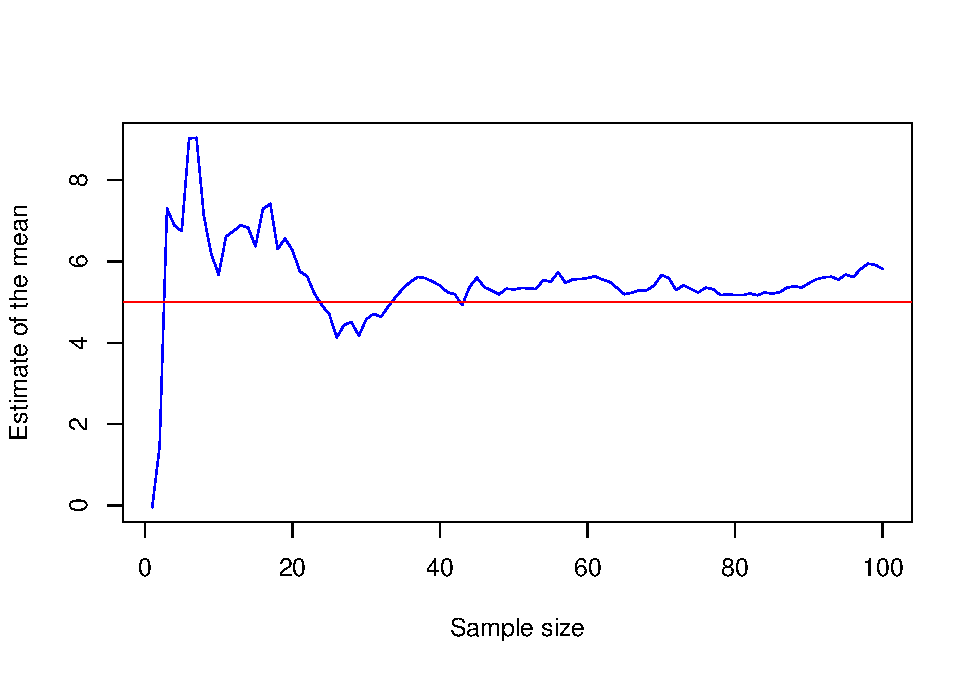
\includegraphics{RMarkdown_files/figure-latex/global_options2-1.pdf}

The plot shows that as the sample size increases, the estimates of the
mean become more accurate and converge to the true mean. At the
beginning, the estimates may deviate substantially from the true mean,
but as the sample size grows, the estimates become more stable and
approach the true mean.

\newpage


\begin{Shaded}
\begin{Highlighting}[]
\NormalTok{knitr}\SpecialCharTok{::}\NormalTok{opts\_chunk}\SpecialCharTok{$}\FunctionTok{set}\NormalTok{(}\AttributeTok{fig.width=}\DecValTok{12}\NormalTok{, }\AttributeTok{fig.height=}\DecValTok{8}\NormalTok{, }\AttributeTok{fig\_path=}\StringTok{\textquotesingle{}figures/\textquotesingle{}}\NormalTok{,}\AttributeTok{echo=}\ConstantTok{TRUE}\NormalTok{, }\AttributeTok{warning=}\ConstantTok{FALSE}\NormalTok{, }\AttributeTok{message=}\ConstantTok{FALSE}\NormalTok{)}

\CommentTok{\# Define parameters}
\NormalTok{mu }\OtherTok{\textless{}{-}} \DecValTok{0}
\NormalTok{sigma }\OtherTok{\textless{}{-}} \DecValTok{1}
\NormalTok{n }\OtherTok{\textless{}{-}} \DecValTok{1000}

\CommentTok{\# Generate two random samples from a standard normal distribution}
\NormalTok{x }\OtherTok{\textless{}{-}} \FunctionTok{rnorm}\NormalTok{(n, }\AttributeTok{mean =}\NormalTok{ mu, }\AttributeTok{sd =}\NormalTok{ sigma)}
\NormalTok{y }\OtherTok{\textless{}{-}} \FunctionTok{rnorm}\NormalTok{(n, }\AttributeTok{mean =}\NormalTok{ mu, }\AttributeTok{sd =}\NormalTok{ sigma)}

\CommentTok{\# Convert the standard normal samples to a Cauchy distribution with scale one}
\NormalTok{z }\OtherTok{\textless{}{-}}\NormalTok{ x }\SpecialCharTok{/}\NormalTok{ y}

\CommentTok{\# Compute estimates of the mean with the first 1, ..., n draws}
\NormalTok{estimates }\OtherTok{\textless{}{-}} \FunctionTok{cumsum}\NormalTok{(z) }\SpecialCharTok{/} \FunctionTok{seq\_along}\NormalTok{(z)}

\CommentTok{\# Plot estimates}
\FunctionTok{plot}\NormalTok{(estimates, }\AttributeTok{type =} \StringTok{"l"}\NormalTok{, }\AttributeTok{col =} \StringTok{"blue"}\NormalTok{, }\AttributeTok{xlab =} \StringTok{"Sample size"}\NormalTok{, }\AttributeTok{ylab =} \StringTok{"Estimate of the mean"}\NormalTok{)}

\CommentTok{\# Add true mean as a horizontal line}
\FunctionTok{abline}\NormalTok{(}\AttributeTok{h =}\NormalTok{ mu, }\AttributeTok{col =} \StringTok{"red"}\NormalTok{)}
\end{Highlighting}
\end{Shaded}

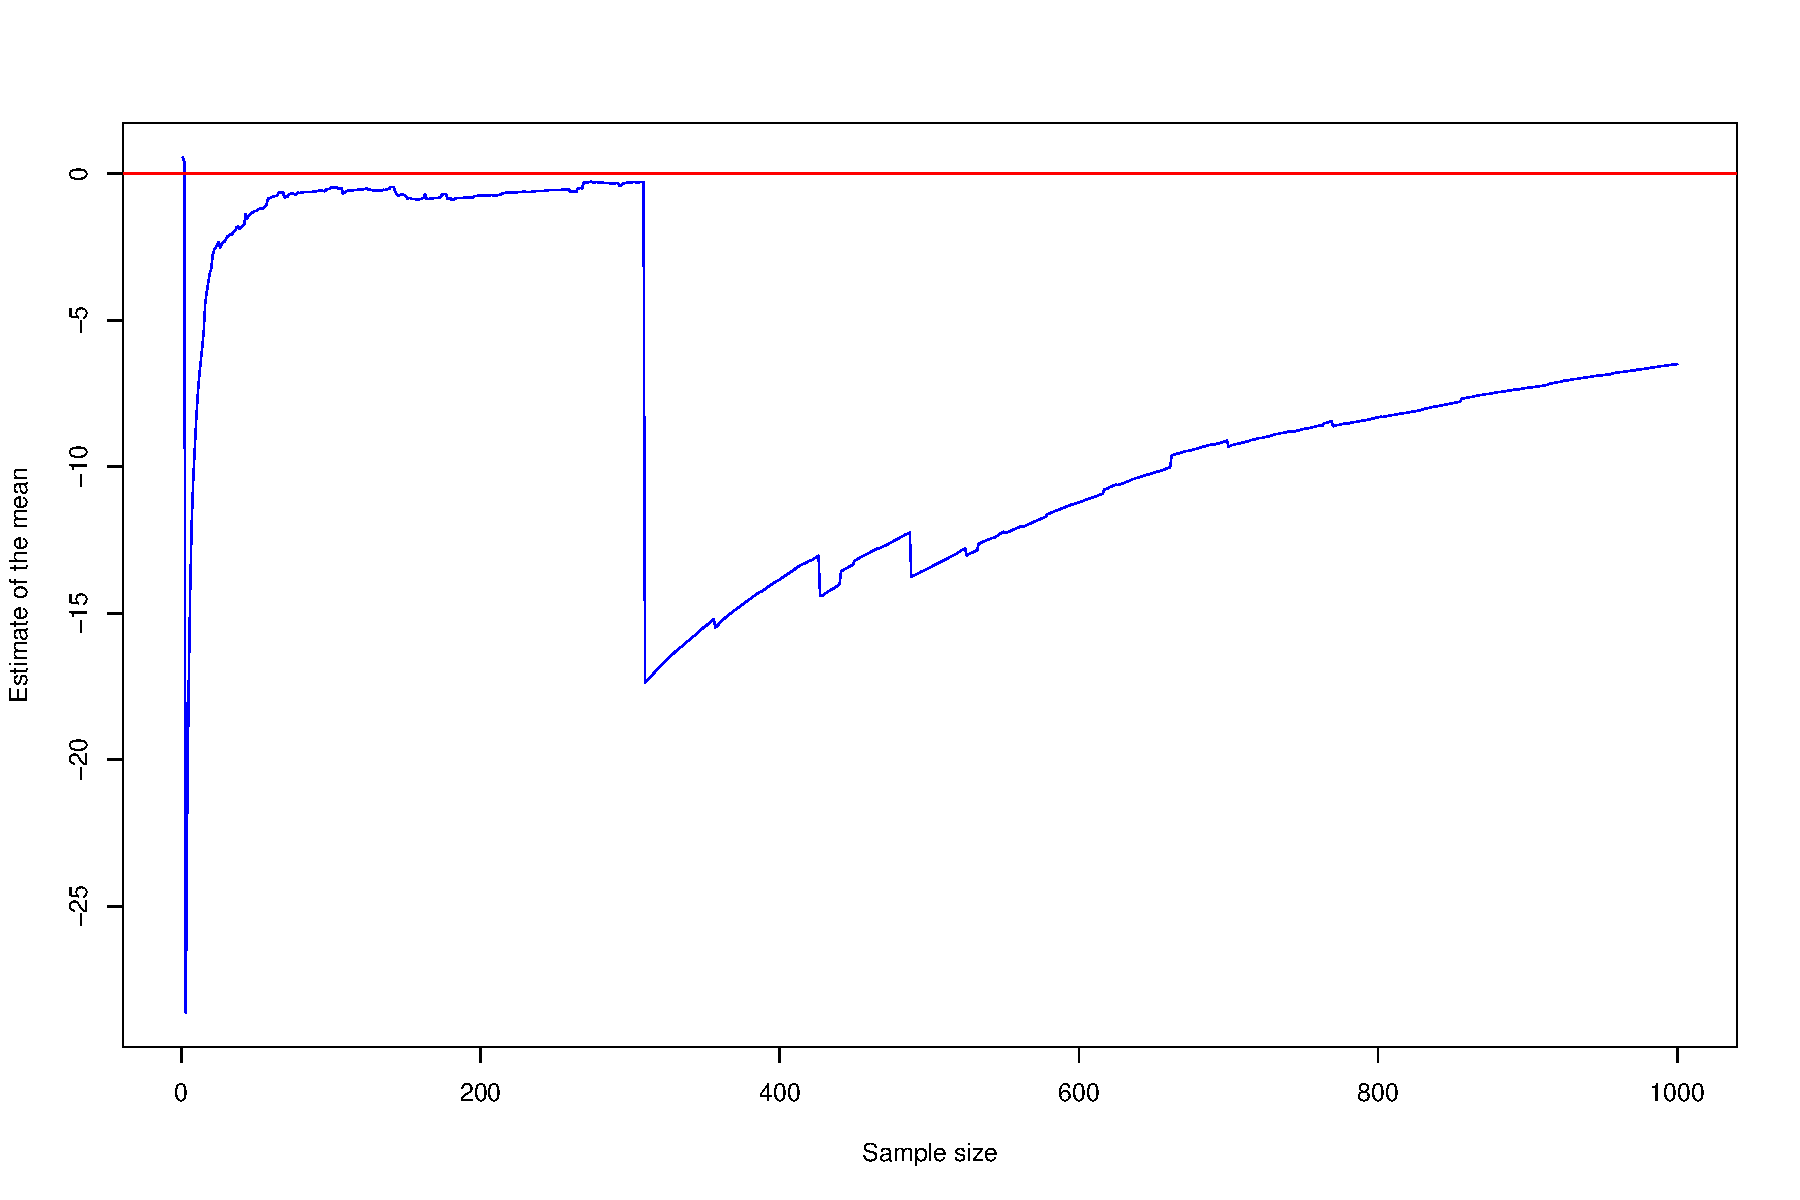
\includegraphics{RMarkdown_files/figure-latex/global_options3-1.pdf}

The Cauchy distribution does not have a well-defined mean and variance,
as its probability density function has ``heavy tails'' that extend to
infinity in both directions. This means that the distribution does not
converge to a particular value as the sample size increases.

\section*{Question 2}

\newpage


\section*{Question 3}

\begin{Shaded}
\begin{Highlighting}[]
\NormalTok{knitr}\SpecialCharTok{::}\NormalTok{opts\_chunk}\SpecialCharTok{$}\FunctionTok{set}\NormalTok{(}\AttributeTok{fig.width=}\DecValTok{12}\NormalTok{, }\AttributeTok{fig.height=}\DecValTok{8}\NormalTok{, }\AttributeTok{fig\_path=}\StringTok{\textquotesingle{}figures/\textquotesingle{}}\NormalTok{,}\AttributeTok{echo=}\ConstantTok{TRUE}\NormalTok{, }\AttributeTok{warning=}\ConstantTok{FALSE}\NormalTok{, }\AttributeTok{message=}\ConstantTok{FALSE}\NormalTok{)}

\CommentTok{\# Question 3}

\NormalTok{simulate\_data }\OtherTok{\textless{}{-}} \ControlFlowTok{function}\NormalTok{(n, k, alpha, beta, sigma) \{}
\NormalTok{  X }\OtherTok{\textless{}{-}} \FunctionTok{matrix}\NormalTok{(}\FunctionTok{rnorm}\NormalTok{(n }\SpecialCharTok{*}\NormalTok{ k, }\AttributeTok{mean =} \DecValTok{0}\NormalTok{, }\AttributeTok{sd =} \DecValTok{1}\NormalTok{), n, k)}
\NormalTok{  epsilon }\OtherTok{\textless{}{-}} \FunctionTok{rnorm}\NormalTok{(n, }\AttributeTok{mean =} \DecValTok{0}\NormalTok{, }\AttributeTok{sd =}\NormalTok{ sigma)}
\NormalTok{  y }\OtherTok{\textless{}{-}}\NormalTok{ alpha }\SpecialCharTok{+}\NormalTok{ X }\SpecialCharTok{\%*\%}\NormalTok{ beta }\SpecialCharTok{+}\NormalTok{ epsilon}
  \FunctionTok{return}\NormalTok{(}\FunctionTok{list}\NormalTok{(}\AttributeTok{X =}\NormalTok{ X, }\AttributeTok{y =}\NormalTok{ y))}
\NormalTok{\}}
\end{Highlighting}
\end{Shaded}



\end{document}




